\documentclass[a4paper,11pt]{article}
\usepackage{geometry}
 \geometry{
 a4paper,
 total={170mm,257mm},
 left=20mm,
 top=20mm,
 }
 \usepackage{colortbl}

 \usepackage{lipsum}  %%% Lorem ipsum

 \setlength{\headheight}{30.0pt}
\setlength{\footskip}{20pt}


 \usepackage[export]{adjustbox}
\usepackage[english]{babel}
\usepackage[utf8]{inputenc}
\usepackage{fancyhdr}
\usepackage{multicol}
\pagestyle{fancy}
\fancyhf{}
\rhead{\textit{Pul074BEX004}}
\lhead{\textit{Amrit Prasad Phuyal}}
\rfoot{\thepage}


\usepackage{mathpazo} % Palatino font
\usepackage{graphicx}
\usepackage{float}

%%%% Anser environment use %%%% Anser environment use %%%% Anser environment use \input{./AnsENV.tex}
%% use \begin{A... {**** argument***}
\RequirePackage{scrextend}

\newenvironment{A}[1]{\textit{Answer:}{\begin{addmargin}[2em]{2em}{#1}\end{addmargin} 
  }}

% just leave some space   
%% use \begin{A... {**** argument***}
\RequirePackage{scrextend}

\newenvironment{A}[1]{\textit{Answer:}{\begin{addmargin}[2em]{2em}{#1}\end{addmargin} 
  }}

% just leave some space   
%% use \begin{A... {**** argument***}
\RequirePackage{scrextend}

\newenvironment{A}[1]{\textit{Answer:}{\begin{addmargin}[2em]{2em}{#1}\end{addmargin} 
  }}

% just leave some space    %% Answer environment 

%%% Question Environment%%%  use 
%%% Question Environment%%%  use 
%%% Question Environment%%%  use \input{./QueENV.tex}   to include
%% Use \begin{Q}....\end{Q}

\newcounter{QC}
\setcounter{QC}{1}
\newenvironment{Q}[1]{
    \section{Question -\arabic{QC}} \stepcounter{QC}{\large\textbf{#1}}
}

%%% Question Environment%%%

   to include
%% Use \begin{Q}....\end{Q}

\newcounter{QC}
\setcounter{QC}{1}
\newenvironment{Q}[1]{
    \section{Question -\arabic{QC}} \stepcounter{QC}{\large\textbf{#1}}
}

%%% Question Environment%%%

   to include
%% Use \begin{Q}....\end{Q}

\newcounter{QC}
\setcounter{QC}{1}
\newenvironment{Q}[1]{
    \section{Question -\arabic{QC}} \stepcounter{QC}{\large\textbf{#1}}
}

%%% Question Environment%%%

 %% Question Environment 
%%%%%% include  Titles.%%%% use \input{./CP}%%%
%%%use """"""""    \CP{}{}{}{}   """" %%%% and 4 argument to craete Title page 
%%%%%%%%%%%%%%%%%%%%%%%%%%%%%%%%%%%%%%%%%%%%%%%%%%%%%%%%%%%%%%%%%
%%%argument number
%% 1=major header ## Course name 
%% 2=minor4 heading ## lab/assignmet no
%% 3=Title  ## Assignment or Lab title
%% 4=submitted to::## input receiver Name"
%%%%%%%%%%%%%%%%%%%%%%%%%%%%%%%%%%%%%%%%%%%%%%%%%%%%%%%%%%%%%%%%%


\usepackage{mathpazo} % Palatino font
\usepackage{graphicx}
\usepackage{float}

%%% format and command for lab ans c and assembly

\newcommand{\HRule}{\rule{\linewidth}{0.4mm}} % Defines a new command for horizontal lines, change thickness here



%----------------------------------------------------------------------------------------
%	TITLE PAGE
%----------------------------------------------------------------------------------------


\newcommand{\CP}[4]{ \begin{titlepage} % Suppresses displaying the page number on the title page and the subsequent page counts as page 1
		%%%%  univerdity logo%%
		\begin{figure}[H]
			\centering
			
\includegraphics[scale=0.13]{tulogo.jpg}
		\end{figure}
		%%% end university logo

		\center % Centre everything on the page

		%------------------------------------------------
		%	Headings
		%------------------------------------------------

		\textsc{\huge Institute of Engineering \\ Central Campus,Pulchowk}\\[1.5cm] % Main heading such as the name of your university/college

		\textsc{\Large #1}\\[0.5cm] % Major heading such as course name

		\textsc{\large #2}\\[0.5cm] % Minor heading such as assignment no./ lab no.

		%------------------------------------------------
		%	Title
		%------------------------------------------------

		\HRule\\[0.4cm]

		{\Huge\bfseries #3}\\[0.4cm] % Title of your document

		\HRule\\[1.5cm]

		%------------------------------------------------
		%	Author(s)
		%------------------------------------------------
		\vfill\vfill
		\begin{minipage}{0.4\textwidth}
			\begin{flushleft}
				\large{
				\textbf{Submitted BY:}\\
				{\normalsize AMRIT PRASAD PHUYAL}\\ % NAME
				{\normalsize Roll: PULL074BEX004}} % Roll
			\end{flushleft}
		\end{minipage}
		~
		\begin{minipage}{0.4\textwidth}
			\begin{flushright}
				\large
				\textbf{Submitted To:}\\
				{ \normalsize{#4}\\ }% recepent's  Name 
				{\normalsize Department of Electronics and Computer Engineering}
			\end{flushright}
		\end{minipage}

		%------------------------------------------------
		%	Date
		%------------------------------------------------

		\vfill\vfill\vfill % Position the date 3/4 down the remaining page

		{\large\today} % Date, change the \today to a set date if you want to be precise

		\vfill % Push the date up 1/4 of the remaining page

	\end{titlepage}
} %%% cover page

%%% For CMD output %%%

%%%%%%%%% use  
%%% For CMD output %%%

%%%%%%%%% use  
%%% For CMD output %%%

%%%%%%%%% use  \include{CMD output.tex}
%%%%%%%%% use \CMD{###filename}{##Caption}
\usepackage{listings}

\usepackage{mdframed}
\usepackage{xcolor}
%\definecolor{codegreen}{rgb}{0,0.6,0}
%\definecolor{codegray}{rgb}{0.4,0.4,0.4}
%\definecolor{codepurple}{rgb}{0.58,0,0.82}
%\definecolor{blackcolour}{rgb}{0,0,0}


\definecolor{bluefront}{RGB}{10,214,255}
\definecolor{blueback}{RGB}{25,24,96}


\renewcommand{\lstlistlistingname}{List of CMD Outputs}
\renewcommand{\lstlistingname}{Output}


\lstdefinestyle{customa}{
    backgroundcolor=\color{blueback},
    %  keywordstyle=\color{magenta},
    %numberstyle=\tiny\color{codegray},
    %stringstyle=\color{codepurple},
    basicstyle=\ttfamily\scriptsize\color{bluefront},
    breakatwhitespace=false,
    breaklines=true,
    captionpos=b,
    %morekeywords={MOV,ADD,ADDC,ACALL,INC,DJNZ,AJMP,RET,END,ORG,RR,JNC,SUBB,JC,DEC},
    keepspaces=true,
    %numbers=left,
    %numbersep=5pt,
    showspaces=false,
    showstringspaces=false,
    showtabs=false,
    tabsize=4
}

\newcommand {\CMD}[2]{

    \begin{mdframed}[backgroundcolor=blueback,innerbottommargin=-2.3em,innertopmargin=-0.1em]
        \lstinputlisting[style=customa,caption={#2}]{#1}
    \end{mdframed}
}

%%% For CMD output %%%


%%%%%%%%% use \CMD{###filename}{##Caption}
\usepackage{listings}

\usepackage{mdframed}
\usepackage{xcolor}
%\definecolor{codegreen}{rgb}{0,0.6,0}
%\definecolor{codegray}{rgb}{0.4,0.4,0.4}
%\definecolor{codepurple}{rgb}{0.58,0,0.82}
%\definecolor{blackcolour}{rgb}{0,0,0}


\definecolor{bluefront}{RGB}{10,214,255}
\definecolor{blueback}{RGB}{25,24,96}


\renewcommand{\lstlistlistingname}{List of CMD Outputs}
\renewcommand{\lstlistingname}{Output}


\lstdefinestyle{customa}{
    backgroundcolor=\color{blueback},
    %  keywordstyle=\color{magenta},
    %numberstyle=\tiny\color{codegray},
    %stringstyle=\color{codepurple},
    basicstyle=\ttfamily\scriptsize\color{bluefront},
    breakatwhitespace=false,
    breaklines=true,
    captionpos=b,
    %morekeywords={MOV,ADD,ADDC,ACALL,INC,DJNZ,AJMP,RET,END,ORG,RR,JNC,SUBB,JC,DEC},
    keepspaces=true,
    %numbers=left,
    %numbersep=5pt,
    showspaces=false,
    showstringspaces=false,
    showtabs=false,
    tabsize=4
}

\newcommand {\CMD}[2]{

    \begin{mdframed}[backgroundcolor=blueback,innerbottommargin=-2.3em,innertopmargin=-0.1em]
        \lstinputlisting[style=customa,caption={#2}]{#1}
    \end{mdframed}
}

%%% For CMD output %%%


%%%%%%%%% use \CMD{###filename}{##Caption}
\usepackage{listings}

\usepackage{mdframed}
\usepackage{xcolor}
%\definecolor{codegreen}{rgb}{0,0.6,0}
%\definecolor{codegray}{rgb}{0.4,0.4,0.4}
%\definecolor{codepurple}{rgb}{0.58,0,0.82}
%\definecolor{blackcolour}{rgb}{0,0,0}


\definecolor{bluefront}{RGB}{10,214,255}
\definecolor{blueback}{RGB}{25,24,96}


\renewcommand{\lstlistlistingname}{List of CMD Outputs}
\renewcommand{\lstlistingname}{Output}


\lstdefinestyle{customa}{
    backgroundcolor=\color{blueback},
    %  keywordstyle=\color{magenta},
    %numberstyle=\tiny\color{codegray},
    %stringstyle=\color{codepurple},
    basicstyle=\ttfamily\scriptsize\color{bluefront},
    breakatwhitespace=false,
    breaklines=true,
    captionpos=b,
    %morekeywords={MOV,ADD,ADDC,ACALL,INC,DJNZ,AJMP,RET,END,ORG,RR,JNC,SUBB,JC,DEC},
    keepspaces=true,
    %numbers=left,
    %numbersep=5pt,
    showspaces=false,
    showstringspaces=false,
    showtabs=false,
    tabsize=4
}

\newcommand {\CMD}[2]{

    \begin{mdframed}[backgroundcolor=blueback,innerbottommargin=-2.3em,innertopmargin=-0.1em]
        \lstinputlisting[style=customa,caption={#2}]{#1}
    \end{mdframed}
}

%%% For CMD output %%%

 %%% Cmd OUTPUT blue background


\begin{document}


%%%%  COver page 
\CP{Computer Network}{Lab \#4}{Subnet Mask, Default Gateway and Static Routing}
{SHARAD KUMAR GHIMIRE}
%%%%%%%%%%%%%%%%%%%%

\pagenumbering{gobble}
\renewcommand{\contentsname}{Table of Contents}
\tableofcontents

%\pagebreak
%\listoffigures
%\pagebreak
%\listoftables
\pagebreak
\lstlistoflistings
\pagebreak
\listoffigures
\pagebreak
\pagenumbering{arabic}

\section{Title} {\large Subnet Mask, Default Gateway and Static Routing}
%%%%%%%%%%%%%%%%%%%%%%%%%%%%
\section{Objective}
\begin{itemize}
      \item To be familiar with network and subnet mask
      \item To be familiar with default gateway and its configuration
      \item To be familiar with Routing: Static Routing and its configuration
\end{itemize}
%%%%%%%%%%%%%%%%%%%%%
\section{Requirement}
\begin{itemize}
      \item Network simulation tool: Packet Tracer
\end{itemize}
%%%%%%%%%%%%%%%%%%%

\section{Procedure}

We created three different networks and explore different networking terms like Subnet, Subnet mask, Default gateway, Routing, Static Routing, Routing table, etc. we also learned the technique to extract network id of destination  network if subnet mask is known.We Configured each interface of each routers. We also explored the telnet through different router and configure it .We performed Numerous Ping operation to confirm the connectivity betweens and among networks and subnets and repeated the Ping operation after configuring the Static route. We also observed the Routing table to confirm the static routing. We have compared the result of previous similar operation/ping with current .

\pagebreak
%%%%%%%%%%%%%%%%%%%%%%%%%%%%%%%%%%%%%%%%%%%%%%%%%%%%%%%%%%%%%%%%%%%%%%%%%%%%%%%%%%%%%%%%%%%%%%%%
\section{Exercises:}
%%%%%%%%%%%%%%%%%%%%%%%%%11111111111111111111111
\begin{Q}
      {
            What is a subnet mask? Why is it used? Explain with examples.
      }
\end{Q}

\begin{A}
      {
      Subnet is a technique to split larger network in to smaller ones like partitioning the whole floor into rooms .If one have to communicate with other on same subnet/Room then  there is no need of Router/doors reducing traffic congestion , unnecessary routes and network speed.

      Subnet mask hides(mask) host id from IP address and is 4 bytes long having similar format to IP address. i.e

      \begin{center}
            \textbf{0-255 . 0-255 . 0-255 . 0-255}
      \end{center}

      Host use subnet mask to determine whether the destination is within the subnet or outside. Subnet mask also serve the purpose of limiting or defining the range of valid ip for specific network.\\

      Lets examine how subnet mask divides network and host id/address from an IP address.
      lets take Class C IP address \textbf{192.168.123.132} and default Class C subnet mask \textbf{255.255.255.0}. here Network id is determined by AND operation of Subnet mask and IP address and remaining part of Ip address is Host id.

      \HRule\\

      {\bfseries

      11000000.10101000.01111011.10000100 -- IP address (192.168.123.132)

      11111111.11111111.11111111.00000000 -- Subnet mask (255.255.255.0)\\


      \textit{ANDing gives Network address and remaning is Host address.\\}


      11000000.10101000.01111011.00000000 -- Network address (192.168.123.0)

      00000000.00000000.00000000.10000100 -- Host address (000.000.000.132)}

      \HRule\\
      }
\end{A}


%%%%%%%%%%%%%%%%%%%%%%%%%%%%%%%%

%%%%%%%%%%%%%%%%%%%%%%%%%2222222222222222222222222222
\begin{Q}
      {
            How does a sending host know whether the destination computer is on the same network or on the different network? How data packet is forwarded in each case from the sending host? Explain.
      }
\end{Q}

\begin{A}
      {
            The Host perform the And operation of it's subnet mask and its IP and then with destination IP and extract and match the network address if matched then it falls on same network if not different.If destination is Local then  host determine the MAC(hardware address) using ARP table and forward the packet to destination directly . If destination is remote then Packet is forwarded to default gateway or Router which then handles the remaining  process by consulting the Routing table to determine the best route to destination.
      }
\end{A}
%%%%%%%%%%%%%%%%%%%%%%%%%%%%%%%%

\pagebreak

%%%%%%%%%%%%%%%%%%%%%%%%%33333333333333333333333333333
\begin{Q}
      {
            What is a routing? Explain static routing and configuration of static routing in a router with its syntax and functions. Also mention how the routing table of a router can be observed.
      }
\end{Q}

\begin{A}
      {
            A Router is a networking device capable of Handling incoming data packets and forwards to their respective destination network after consulting routing table.
            Routing is technique of selecting the best route for data packets to destination.

            Static Routing is the Non adaptive and manual way of adding routes in Routing table of the Router.Here the routes are fixed by administrator abd unaffected by any changes in network topology.It is easy to configure , Secure and less resource consuming.However it is not suitable for large network and one need to have sound knowledge of topology to configure static routing.


            The basic syntax for static routing Configuration is :
            \begin{center}
                  {\bfseries \textit {ip route}  \quad Destination-Network \quad  Subnet-Mask   \quad   [next-hop-address or outgoing interface]}
            \end{center}

            \begin{itemize}
                  \item Destination Network: Destination Network address
                  \item Subnet-mask: only needed if subnetting is implemented and used tto reveal the destination network address.
                  \item Next-hop-address or outgoing interface: Its an Ip of nearest Router in Routing Path or alternatively we can also specify the interface.

                        There are other parameters like administrative distance and Permanent.
            \end{itemize}
      }
      The Routing Table of router can be observed using command {\bfseries \textit{show ip route} }

\end{A}
%%%%%%%%%%%%%%%%%%%%%%%%%%%%%%%%

%%%%%%%%%%%%%%%%%%%%%%%%%4444444444444444444
\begin{Q}
      {
            Note down the observation of each steps with necessary commands specified in activities A, B and C mentioned above and comment on it.\\
      }
\end{Q}


%%%%%%%%%%%%%%%%%%%%%%AAAAAAAAAAAAAAAAAAAAAAAAAAAAAAAA
{\bfseries \textit{A. Create the following network topology using Packet Tracer and perform the followings:}}

\begin{figure}[H]
      \centering
      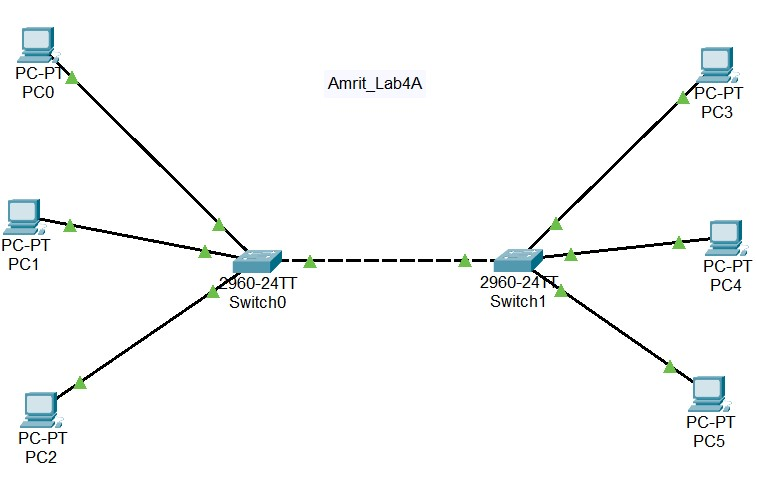
\includegraphics[scale=0.80,cframe=blue 0.5pt 3pt]{Lab4A.jpg}
      \caption{Network topology Lab 4A}
\end{figure}

\begin{enumerate}
      %%%%%%%%%%%%%%%%%%%%AAAAAAAAAAAAAAAAA11111111111111
      \item \textbf{Assign the IP Address and subnet mask of given computers as:}
            It is performed using the GUI interface available in every PC
            \begin{itemize}
                  \item  PC0: 200.200.20.2 \quad \quad 255.255.255.0
                        \begin{figure}[H]
                              \centering
                              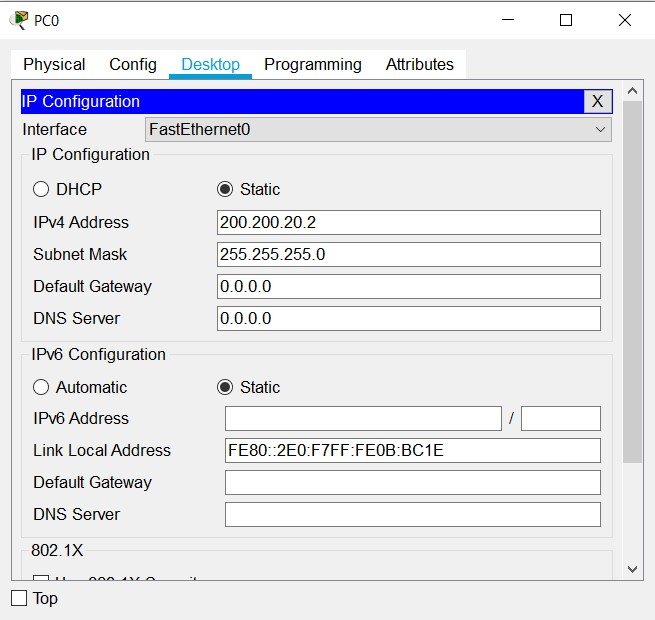
\includegraphics[scale=0.8,cframe=blue 0.5pt 3pt]{PC0 ip sub.jpg}
                              \caption{PC0 IP configuration}
                        \end{figure}
                  \item PC1: 200.200.20.3 \quad \quad 255.255.255.0
                  \item PC2: 200.200.20.4 \quad \quad 255.255.255.0
                  \item PC3: 200.200.20.34 \quad \quad 255.255.255.0
                  \item PC4: 200.200.20.35 \quad \quad 255.255.255.0
                  \item PC5: 200.200.20.36 \quad \quad 255.255.255.0
            \end{itemize}
            %%%%%%%%%%%%%%%%%%%%%%%%%%%%%%%%%%%AAAAAAAAAAAAAAAAAAAA222222222222222222
      \item \textbf{Test the connectivity from PC0 to each of the following computers one by one using ping command and note down the result.}
            \begin{itemize}
                  \item PC1: Ping Successful
                        \addtocontents{lol}{\protect\subsection*{Activities A}}
                        \CMD{AP0-1.txt}{Ping PC0 to PC1}
                        \textit{Similarly for all PCs ping  is performed and result is noted}\\
                  \item PC2: Ping Successful
                  \item PC3: Ping Successful
                  \item PC4: Ping Successful
                  \item PC5: Ping Successful
            \end{itemize}
            %%%%%%%%%%%%%%%%%%%%%%%%%%%%AAAAAAAAAAAAA333333333333333333
      \item \textbf{Again, test the connectivity from PC3 to each of the following computers one by one using ping command and note down the result.}

            \begin{itemize}
                  \item PC0: Ping Successful
                        \CMD{AP3-0.txt}{Ping PC3 to PC0}
                        \textit{Similarly for all PCs ping  is performed and result is noted}\\
                  \item PC1: Ping Successful
                  \item PC2: Ping Successful
                  \item PC4: Ping Successful
                  \item PC5: Ping Successful
            \end{itemize}
            %%%%%%%%%%%%%%%%%%%%%%%%AAAAAAAAAAAA4444444444444444444444444444
      \item \textbf{Change the subnet mask of each of the computer as: 255.255.255.224. Now again test the connectivity from PC0 to each of the following computers one by one using ping command and note down the result.}

            \begin{itemize}
                  \item PC1: Ping Successful
                        \CMD{APS0-1.txt}{Ping PC0 to PC1}
                  \item PC2: Ping Successful\\

                  \item PC3: Ping Failed
                        \CMD{APS0-3.txt}{Ping PC0 to PC3}
                  \item PC4: Ping Failed
                  \item PC5: Ping Failed
            \end{itemize}

            In \textbf{A.2} PC0 could ping all the computers from PC0 to PC6 but now it is unable to ping Network 2 i.e PC3,PC4,PC5  due to Change in Subnet mask. Previously the default subnet mask \textbf{255.255.255.0} due to which Both network 1 and 2 has Network address as \textbf{200.200.20.0} and acts as single network and can forwards packets within the networks freely. But when subnet mask is changed to \textbf{255.255.255.224} the network splits into subnet and network address for Network 1 becomes \textbf{200.200.20.0} and for Network 2 it is \textbf{200.200.20.32}.  So they became the different network and as we know we need Router and Routing Routes to properly exchange package between networks.

            The process to obtain Network address is explained in Exercise 1 and the detailed process of obtaining Network Id for both Network is explained in Activities C.11


            %%%%%%%%%%%%%%%%%%%%%%AAAAAAAAAAAAAAAAAAAAA55555555555555555
      \item \textbf{Again, test the connectivity from PC3 to each of the following computers one by one using ping command and note down the result.}
            \begin{itemize}
                  \item PC0: Ping Failed
                        \CMD{APS3-0.txt}{Ping PC3 to PC0}
                  \item PC1: Ping Failed
                  \item PC2: Ping Failed\\
                  \item PC4: Ping Successful
                        \CMD{APS3-4.txt}{Ping PC3 to PC4}
                  \item PC5: Ping Successful\\
            \end{itemize}
            In \textbf{A.3} PC3 could ping all the computers from PC0 to PC6 but now it is unable to ping Network 1 i.e PC0,PC1,PC2  due to Change in Subnet mask. Previously the default subnet mask \textbf{255.255.255.0} due to which Both network 1 and 2 has Network address as \textbf{200.200.20.0} and acts as single network and can forwards packets within the networks freely. But when subnet mask is changed to \textbf{255.255.255.224} the network splits into subnet and network address for Network 1 becomes \textbf{200.200.20.0} and for Network 2 it is \textbf{200.200.20.32}.  So they became the different network and as we know we need Router and Routing Routes to properly exchange package between networks.

            The process to obtain Network address is explained in Exercise 1 and the detailed process of obtaining Network Id for both Network is explained in Activities C.11

\end{enumerate}


\pagebreak

%%%%%%%%%%%%%%%%%%%%%BBBBBBBBBBBBBBBBBBBBBBBBBBBBBBBBBBBBBBB
{\bfseries \textit{B. Modify the above network as following i.e. use a router in between switches (i.e. between Switch1 and Switch2), and perform the followings::}}

\begin{figure}[H]
      \centering
      \includegraphics[scale=0.60,cframe=blue 0.5pt 3pt]{Lab4B.jpg}
      \caption{Network topology Lab 4B}
\end{figure}

\begin{enumerate}
      %%%%%%%%%%%%%%%%BBBBBBBBBBBBBBBBB111111111111111111111111
      \item \textbf{Assign the IP address of GigabitEthernet 0/0 interface of Router0 as 200.200.20.1 255.255.255.224 and turn on the interface. Similarly assign the IP address of GigabitEthernet 0/1 interface of Router0 as 200.200.20.33 255.255.255.224 and turn on the interface.}

            \addtocontents{lol}{\protect\subsection*{Activities B}}
            \CMD{IP00.txt}{Assign the IP address of GigabitEthernet 0/0 for Router 0}
            \CMD{IP01.txt}{Assign the IP address of GigabitEthernet 0/1 for Router 0}



            %%%%%%%%%%%%%%%%%%%BBBBBBBBBBBBBBBBB2222222222222222222222
      \item \textbf{Now test the connectivity from PC0 to each of the following computers one by one using ping command and note down the result and comment on it.}
            \begin{itemize}
                  \item PC1: Ping Successful
                        \CMD{BP0-1.txt}{Ping PC0 to PC1}
                  \item PC2: Ping Successful\\
                  \item PC3: Ping Failed
                        \CMD{BP0-3.txt}{Ping PC0 to PC3}
                  \item PC4: Ping Failed
                  \item PC5: Ping Failed
            \end{itemize}
            %%%%%%%%%%%%%%%%%%%%%BBBBBBBBBBBBBBBBBBBB3333333333333333333
      \item \textbf{Now again, test the connectivity from PC3 to each of the following computers one by one using ping command and note down the result and comment on it.}
            \begin{itemize}
                  \item PC0: Ping Failed
                        \CMD{BP3-0.txt}{Ping PC3 to PC0}
                  \item PC1: Ping Failed
                  \item PC2: Ping Failed\\
                  \item PC4: Ping Successful
                        \CMD{BP3-4.txt}{Ping PC3 to PC4}
                  \item PC5: Ping Successful
            \end{itemize}

            %%%%%%%%%%%%%%%%%%%%BBBBBBBBBBBBBBBBBBBBBBBBBBBBBBBB4444444444444444444444444444

      \item \textbf{Assign the default gateway of 200.200.20.1 on PC0, PC1 and PC2. Similarly assign default gateway of 200.200.20.33 on PC3, PC4 and PC5. Again test the connectivity from PC0 to each of the following computers one by one using ping command and note down the result.}
            \begin{itemize}
                  \item PC1: Ping Successful
                        \CMD{BPG0-1.txt}{Ping PC0 to PC1}
                  \item PC2: Ping Successful\\
                  \item PC3: Ping Successful
                        \CMD{BPG0-3.txt}{Ping PC0 to PC3}
                  \item PC4: Ping Successful
                  \item PC5: Ping Successful
            \end{itemize}

            In Activity \textbf{B.2} PC0 could ping only the PCs in it's Network and unable to ping PCs on Network 2. This is because the default gateway was set to \textbf{0.0.0.0} so when PC0 try to connect to PCs on other Network PC0 extract the network id and since they belongs to different network , a Router is needed to establish the connection.
            Since default gateway is set to \textbf{0.0.0.0} all outgoing package is forwarded to unknown address which never reach the destination.

            But this all changes once correct Default gateway is set for all PCs in both network . For network 1 default gateway is set to \textbf{200.200.20.1} and for Network 2 \textbf{200.200.20.33}.Since Default gateway is set  both Network can successfully pass the outgoing packet to Router and communicate with each other.So in this activity PC0 could ping all other PCs.


            %%%%%%%%%%%%%%%%%%%%%%%%%%%%%%%%%%%BBBBBBBBBBBBBBBBBBBBBBB555555555555555555555555
      \item \textbf{Now again, test the connectivity from PC3 to each of the following computers one by one using ping command and note down the result and comment on it.}
            \begin{itemize}
                  \item PC0: Ping Successful
                        \CMD{BPG3-0.txt}{Ping PC3 to PC0}
                  \item PC1: Ping Successful
                  \item PC2: Ping Successful\\
                  \item PC4: Ping Successful
                        \CMD{BPG3-4.txt}{Ping PC3 to PC4}
                  \item PC5: Ping Successful
            \end{itemize}


            In Activity \textbf{B.2} PC3 could ping only the PCs in it's Network and unable to ping PCs on Network 2. This is because the default gateway was set to \textbf{0.0.0.0} so when PC0 try to connect to PCs on other Network PC3 extract the network id and since they belongs to different network , a Router is needed to establish the connection.
            Since default gateway is set to \textbf{0.0.0.0} all outgoing package is forwarded to unknown address which never reach the destination.

            But this all changes once correct Default gateway is set for all PCs in both network . For network 1 default gateway is set to \textbf{200.200.20.1} and for Network 2 \textbf{200.200.20.33}.Since Default gateway is set  both Network can successfully pass the outgoing packet to Router and communicate with each other.So in this activity PC3 could ping all other PCs.

            %%%%%%%%%%%%%%%%%BBBBBBBBBBBBBBBBBBBBBBBBB66666666666666666666666
      \item \textbf{Use the command \textit{show ip route} in the router and note down the result, and comment on it.}
            \CMD{showip.txt}{\textit{show ip route}}

\end{enumerate}

\pagebreak
%%%%%%%%%%%%%%%%%%%%%%%%%%%%%%%%%%%%%%%%%%%%CCCCCCCCCCCCCCCCCCCCCCCCCCCCCCCCCCCCCCCC
{\bfseries \textit{C. Modify the above network to connect additional networks by using another router as following,and perform the followings:}}
\begin{figure}[H]
      \centering
      \includegraphics[scale=0.70,cframe=blue 0.5pt 3pt]{Lab4C.jpg}
      \caption{Network topology Lab 4C}
\end{figure}

\begin{enumerate}
      %%%%%%%%%%%%%%%%%%%%%%%%CCCCCCCCCCCCCCCCCCCCCC1111111111111111111111111111
      \item \textbf{Assign default gateway for each computer as 200.200.20.99 and Assign the IP Address and subnet mask of added computers as:}
            \begin{itemize}
                  \item PC6: 200.200.20.100\quad \quad 255.255.255.224
                        \begin{figure}[H]
                              \centering
                              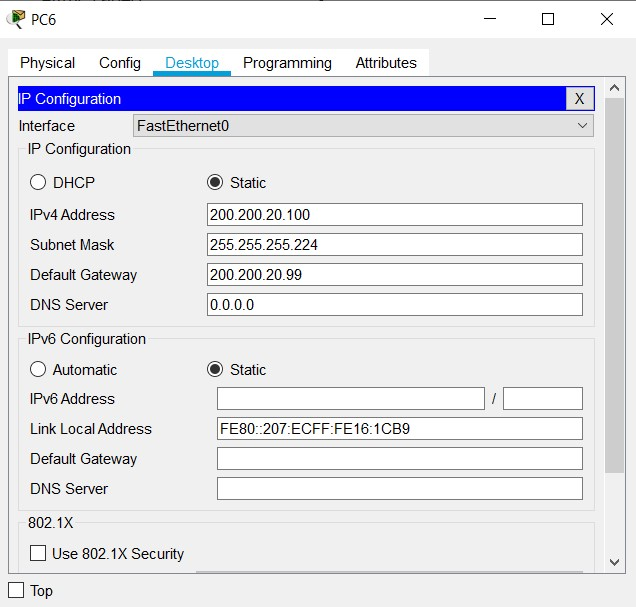
\includegraphics[scale=0.75,cframe=blue 0.5pt 3pt]{gate_ip_mask.jpg}
                              \caption{Assign default gateway, ip and subnet mask}
                        \end{figure}
                  \item PC7: 200.200.20.101\quad \quad 255.255.255.224
                  \item PC8: 200.200.20.102\quad \quad 255.255.255.224
            \end{itemize}


            %%%%%%%%%%%%%%%%%%%%%%%%%%%%%%%%%%CCCCCCCCCCCCCCCCCCCCCCC222222222222222222222222
      \item \textbf{Also configure the GigabitEthernet interfaces of routers with following IP Addresses and turn on the corresponding interfaces.}

            \begin{itemize}
                  \item Router0: GigabitEthernet 0/2 200.200.20.65 255.255.255.224
                        \addtocontents{lol}{\protect\subsection*{Activities C}}
                        \addtocontents{lol}{\protect\subsubsection*{C.2}}
                        \CMD{IP002.txt}{Assign the IP address of GigabitEthernet 0/2 for Router 0}

                  \item Router1: GigabitEthernet 0/0 200.200.20.66 255.255.255.224
                        \CMD{IP100.txt}{Assign the IP address of GigabitEthernet 0/0 for Router 1}

                  \item Router1: GigabitEthernet 0/1 200.200.20.99 255.255.255.224
                        \CMD{IP101.txt}{Assign the IP address of GigabitEthernet 0/1 for Router 1}
            \end{itemize}

            %%%%%%%%%%%%%%%%%%%%%%%%%%%%%%%%%%CCCCCCCCCCCCCCCCCCCCCCC33333333333333333
      \item \textbf{Configure the hostname, console password, vty password and enable password in both routers. Hostname of Router0 should be your first name and hostname of Router1 should be your surname. Set console password as your first name, enable password as your roll no. like 456 and vty password as your surname for each router.}

            \begin{table}[H]
                  \centering
                  \begin{tabular}{|l|l|l|l|l|}
                        \hline
                        \rowcolor[rgb]{0.424,0.412,0.925} {\cellcolor[rgb]{0.255,0.824,0.576}}S.N & Hostname & Console Password & Enable Password & Vty Password \\
                        \hline
                        {\cellcolor[rgb]{0.255,0.824,0.576}}Router 0                              & AMRIT    & amrit            & 403             & phuyal       \\
                        \hline
                        {\cellcolor[rgb]{0.255,0.824,0.576}}Router 1                              & Phuyal   & amrit            & 403             & phuyal       \\
                        \hline
                  \end{tabular}
            \end{table}
            \addtocontents{lol}{\protect\subsubsection*{C.3}}
            \CMD{config0.txt}{Configuration for Router 0}
            \CMD{config1.txt}{Configuration for Router 1}

            %%%%%%%%%%%%%%%%%%%%%%%%%%%%%%%%%%CCCCCCCCCCCCCCCCCCCCCCC44444444444444444444
      \item \textbf{Observe and note down the output of the command \textit{show ip route} in each router.}

            \addtocontents{lol}{\protect\subsubsection*{C.4}}
            \CMD{showip0.txt}{\textit{show ip route} Router 0}
            \CMD{showip1.txt}{\textit{show ip route} Router 1}

            %%%%%%%%%%%%%%%%%%%%%%%%%%%%%%%%%%CCCCCCCCCCCCCCCCCCCCCCC55555555555555555555
            %%%%%%%%%%%%%%%TABLE Showing ALL Assigned IPs
            % \usepackage{colortbl}


            \begin{table}[H]
                  \centering
                  \begin{tabular}{| m{15em}| m{9em}|}
                        \hline
                        {\cellcolor[rgb]{0.324,0.553,0.912}} \textbf{Name } & \textbf
                        {IP}                                                                 \\
                        \hline
                        {\cellcolor[rgb]{0.324,0.553,0.912}}PC0             & 200.200.20.2   \\
                        \hline
                        {\cellcolor[rgb]{0.324,0.553,0.912}}PC1             & 200.200.20.3   \\
                        \hline
                        {\cellcolor[rgb]{0.324,0.553,0.912}}PC2             & 200.200.20.4   \\
                        \hline
                        {\cellcolor[rgb]{0.324,0.553,0.912}}{Router 0 0/0}  & 200.200.20.1   \\
                        \hline
                        {\cellcolor[rgb]{0.324,0.553,0.912}}{Router 0 0/1}  & 200.200.20.33  \\
                        \hline
                        {\cellcolor[rgb]{0.324,0.553,0.912}}{Router 0 0/2}  & 200.200.20.65  \\
                        \hline
                        {\cellcolor[rgb]{0.324,0.553,0.912}}PC3             & 200.200.20.34  \\
                        \hline
                        {\cellcolor[rgb]{0.324,0.553,0.912}}PC4             & 200.200.20.35  \\
                        \hline
                        {\cellcolor[rgb]{0.324,0.553,0.912}}PC5             & 200.200.20.36  \\
                        \hline
                        {\cellcolor[rgb]{0.324,0.553,0.912}}{Router 1 0/0}  & 200.200.20.66  \\
                        \hline
                        {\cellcolor[rgb]{0.324,0.553,0.912}}{Router 1 0/1}  & 200.200.20.99  \\
                        \hline
                        {\cellcolor[rgb]{0.324,0.553,0.912}}PC6             & 200.200.20.100 \\
                        \hline
                        {\cellcolor[rgb]{0.324,0.553,0.912}}PC7             & 200.200.20.101 \\
                        \hline
                        {\cellcolor[rgb]{0.324,0.553,0.912}}PC8             & 200.200.20.102 \\
                        \hline
                  \end{tabular}
            \end{table}


      \item \textbf{Observe the output while using ping command from PC0 to PC0, PC1, PC2, PC3, PC4, PC5, PC6, PC7, PC8, Router0 and Router1 (use each IP address of router).}
            \begin{itemize}
                  \item PC0: Ping Successful
                  \item PC1: Ping Successful
                  \item PC2: Ping Successful
                  \item Router 0 0/0: Ping Successful
                        \addtocontents{lol}{\protect\subsubsection*{C.5}}
                        \CMD{CP0-r00.txt}{Ping PC0 to Router 0 0/0}
                  \item Router 0 0/1: Ping Successful
                  \item Router 0 0/2: Ping Successful
                        \CMD{CP0-r02.txt}{Ping PC0 to Router 0 0/2}
                  \item PC3: Ping Successful
                  \item PC4: Ping Successful
                  \item PC5: Ping Successful
                  \item Router 1 0/0: Ping Failed (Request timed out)
                        \CMD{CP0-r10.txt}{Ping PC0 to Router 1 0/0}
                  \item Router 1 0/1: Ping Failed (Destination host unreachable)
                        \CMD{CP0-r11.txt}{Ping PC0 to Router 1 0/1}
                  \item PC6: Ping Failed (Destination host unreachable)
                        \CMD{CP0-6.txt}{Ping PC0 to PC6}
                  \item PC7: Ping Failed (Destination host unreachable)
                  \item PC8: Ping Failed (Destination host unreachable)
            \end{itemize}



            %%%%%%%%%%%%%%%%%%%%%%%%%%%%%%%%%%CCCCCCCCCCCCCCCCCCCCCCC666666666666666666666666
      \item \textbf{Observe the output while using ping command from PC3 to PC0, PC1, PC2, PC3, PC4, PC5, PC6, PC7, PC8, Router0 and Router1 (use each IP address of router).}
            \begin{itemize}
                  \item PC0: Ping Successful
                  \item \addtocontents{lol}{\protect\subsubsection*{C.6}}
                        \CMD{CP3-0.txt}{Ping PC3 to PC0}

                  \item PC1: Ping Successful
                  \item PC2: Ping Successful
                  \item Router 0 0/0: Ping Successful
                  \item Router 0 0/1: Ping Successful
                  \item Router 0 0/2: Ping Successful
                        \CMD{CP3-r02.txt}{Ping PC3 to Router 0 0/2}
                  \item PC3: Ping Successful
                  \item PC4: Ping Successful
                  \item PC5: Ping Successful
                  \item Router 1 0/0: Ping Failed (Request timed out)
                        \CMD{CP3-r10.txt}{Ping PC3 to Router 1 0/0}
                  \item Router 1 0/1: Ping Failed (Destination host unreachable)
                        \CMD{CP3-r11.txt}{Ping PC3 to Router 1 0/1}
                  \item PC6: Ping Failed (Destination host unreachable)
                        \CMD{CP3-6.txt}{Ping PC3 to PC6}
                  \item PC7: Ping Failed (Destination host unreachable)
                  \item PC8: Ping Failed (Destination host unreachable)
            \end{itemize}

            %%%%%%%%%%%%%%%%%%%%%%%%%%%%%%%%%%CCCCCCCCCCCCCCCCCCCCCCC77777777777777777777
      \item \textbf{Observe the output while using ping command from PC6 to PC0, PC1, PC2, PC3, PC4, PC5, PC6, PC7, PC8, Router0 and Router1 (use each IP address of router).}
            \begin{itemize}
                  \item PC0: Ping Failed (Destination host unreachable)

                  \item PC1: Ping Failed (Destination host unreachable)
                        \addtocontents{lol}{\protect\subsubsection*{C.7}}
                        \CMD{CP6-1.txt}{Ping PC6 to PC1}
                  \item PC2: Ping Failed (Destination host unreachable)
                  \item Router 0 0/0: Ping Failed (Destination host unreachable)
                  \item Router 0 0/1: Ping Failed (Destination host unreachable)
                        \CMD{CP6-r01.txt}{Ping PC6 to Router 0 0/1}
                  \item Router 0 0/2: Ping Failed (Request timed out)
                  \item \CMD{CP6-r02.txt}{Ping PC6 to Router 0 0/2}
                  \item PC3: Ping Failed (Destination host unreachable)
                  \item PC4: Ping Failed (Destination host unreachable)
                  \item PC5: Ping Failed (Destination host unreachable)
                  \item Router 1 0/0: Ping Successful
                  \item \CMD{CP6-r10.txt}{Ping PC6 to Router 1 0/0}
                  \item Router 1 0/1: Ping Successful
                  \item \CMD{CP6-r11.txt}{Ping PC6 to Router 1 0/1}
                  \item PC6: Ping Successful
                  \item PC7: Ping Successful
                  \item PC8: Ping Successful
            \end{itemize}

            %%%%%%%%%%%%%%%%%%%%%%%%%%%%%%%%%%CCCCCCCCCCCCCCCCCCCCCCC888888888888888888888
      \item \textbf{Observe the output while using ping command from Router0 to PC0, PC1, PC2, PC3, PC4, PC5, PC6, PC7, PC8 and Router1 (use each IP address of router).}
            \begin{itemize}
                  \item PC0: Ping Successful

                  \item PC1: Ping Successful
                        \addtocontents{lol}{\protect\subsubsection*{C.8}}
                        \CMD{CR0-1.txt}{Ping Router 0 to PC1}
                  \item PC2: Ping Successful
                  \item PC3: Ping Successful
                        \CMD{CR0-3.txt}{Ping Router 0 to PC3}
                  \item PC4: Ping Successful
                  \item PC5: Ping Successful
                  \item Router 1 0/0: Ping Successful
                        \CMD{CR0-r10.txt}{Ping Router 0 to Router 1 0/0}
                  \item Router 1 0/1: Ping Failed
                        \CMD{CR0-r11.txt}{Ping Router 0 to Router 1 0/1}
                  \item PC6: Ping Failed
                        \CMD{CR0-6.txt}{Ping Router 0 to PC6}
                  \item PC7: Ping Failed
                  \item PC8: Ping Failed
            \end{itemize}

            %%%%%%%%%%%%%%%%%%%%%%%%%%%%%%%%%%CCCCCCCCCCCCCCCCCCCCCCC99999999999999999999
      \item \textbf{Observe the output while using ping command from Router1 to PC0, PC1, PC2, PC3, PC4, PC5, PC6, PC7, PC8 and Router0 (use each IP address of router).}
            \begin{itemize}
                  \item PC0: Ping Failed
                        \addtocontents{lol}{\protect\subsubsection*{C.9}}
                        \CMD{CR1-0.txt}{Ping Router 1 to Router PC0}
                  \item PC1: Ping Failed
                        \CMD{CR1-1.txt}{Ping Router 1 to PC1}
                  \item PC2: Ping Failed
                  \item Router 0 0/0: Ping Failed
                  \item Router 0 0/1: Ping Failed
                  \item Router 0 0/2: Ping Successful
                        \CMD{CR1-r02.txt}{Ping Router 1 to Router 0 0/2}
                  \item PC3: Ping Failed
                        \CMD{CR1-3.txt}{Ping Router 1 to PC3}
                  \item PC4: Ping Failed
                  \item PC5: Ping Failed
                  \item PC6: Ping Successful
                        \CMD{CR1-6.txt}{Ping Router 1 to PC6}
                  \item PC7: Ping Successful
                  \item PC8: Ping Successful
            \end{itemize}

            %%%%%%%%%%%%%%%%%%%%%%%%%%%%%%%%%%CCCCCCCCCCCCCCCCCCCCCCC10 10 10 10 10 10 10 10
      \item \textbf{From PC0 enter into Router0 using telnet and configure the static route for destination network of  Network 3.}

            For Static \textit{ip route} command is used and syntax is:
            \begin{center}
                  {\bfseries \textit {ip route}  \quad Destination-Network \quad  Subnet-Mask   \quad   [next-hop-address or outgoing interface]}
            \end{center}

            We are aware of Subnet mask  and next-hop-address but unknown to Destination-network. which we have to calculate by ANDing the IP address's of network and assigned subnet mask for that network. For Network 3 assigned IPs are 200.200.20.100, 200.200.20.101 and  200.200.20.102 so by ANDing any of these IP with Subnet mask \textbf{255.255.255.224} we get Destination-network.

            \HRule\\
            {\bfseries 11001000.11001000.00010100.011 00101 -- IP address (200.200.20.101)\\
            11111111.11111111.11111111.111 00000 -- Subnet mask (255.255.255.224)\\


            \textit{ANDing gives Network address .\\}


            11001000.11001000.00010100.011 00000 -- Network address (200.200.20.96)\\}

            \HRule\\

            Net hop address is the address of closet router in routing path to travel from router 0 to router 1 next hop address is \textbf{200.200.20.66}. So the syntax will be :
            \begin{center}
                  \textit{ip route \quad 200.200.20.96 \quad 255.255.255.224 \quad 200.200.20.66}
            \end{center}

            \addtocontents{lol}{\protect\subsubsection*{C.10}}

            \CMD{CT0-r0.txt}{Telnet to Router 0 and configure for static route for net 3 }




            %%%%%%%%%%%%%%%%%%%%%%%%%%%%%%%%%%CCCCCCCCCCCCCCCCCCCCCCC11 11 11 11 11 11 
      \item \textbf{From there enter into Router1 using telnet and configure the static route for destination network of Network 1 and Network 2.}

            Without existing from telnet we further telnet to Router 1 to configure Static Route for network 1 and 2. The Destination address for network 1 is calculated as :

            %%%%%%%%%%%%%%%%%%%%%network 1
            \HRule\\
            {\bfseries 11001000.11001000.00010100.000 00011 -- IP address (200.200.20.3)\\
            11111111.11111111.11111111.111 00000 -- Subnet mask (255.255.255.224)\\


            \textit{ANDing gives Network address.\\}


            11001000.11001000.00010100.000 00000 -- Network address (200.200.20.0)\\}

            \HRule\\


            %%%%%%%%%%%%%%%%%%%%%network 2
            Similarly,The Destination address for network 2 is calculated as :\\
            \HRule\\
            {\bfseries  11001000.11001000.00010100.001 00011 -- IP address (200.200.20.35)\\
            11111111.11111111.11111111.111 00000 -- Subnet mask (255.255.255.224)\\


            \textit{ANDing gives Network address .\\}


            11001000.11001000.00010100.001 00000 -- Network address (200.200.20.32)\\}
            \HRule\\


            Thus destination address for Network 1 is \textbf{200.200.20.0} and for network 2 is \textbf{200.200.20.32}. The next hop address for both network is same i.e. \textbf{200.200.20.65}.


            \addtocontents{lol}{\protect\subsubsection*{C.11}}
            \CMD{CT0-r0-r1.txt}{Telnet to Router 1 and configure for static route for net 1 and 2}



            %%%%%%%%%%%%%%%%%%%%%%%%%%%%%%%%%%CCCCCCCCCCCCCCCCCCCCCCC12 12 12 12 12 12 12 12 
      \item \textbf{Repeat the step from 4 to 9 and observe the output. Compare the result with previous and comment on it.}

            \textbf{.Observe and note down the output of the command show ip route in each router.}
            \addtocontents{lol}{\protect\subsubsection*{Activities C :Repeating exercise C4-C9 after configuring Static route}}

            We can observe the added Static routes  in routing table of Router 0 and Router 1.

            \CMD{Sshowip0.txt}{\textit{show ip route} Router 0 after static route}
            \CMD{Sshowip1.txt}{\textit{show ip route} Router 1 after static route}

            \begin{itemize}
                  \item \textbf{Observe the output while using ping command from PC0 to PC0, PC1, PC2, PC3, PC4, PC5, PC6,
                              PC7, PC8, Router0 and Router1 (use each IP address of router).}
                        \begin{itemize}
                              \item PC0: Ping Successful
                              \item PC1: Ping Successful
                              \item PC2: Ping Successful
                              \item Router 0 0/0: Ping Successful
                              \item Router 0 0/1: Ping Successful
                              \item Router 0 0/2: Ping Successful
                              \item PC3: Ping Successful
                              \item PC4: Ping Successful
                              \item PC5: Ping Successful
                              \item Router 1 0/0: Ping Successful
                              \item Router 1 0/1: Ping Successful
                              \item PC6: Ping Successful
                                    \CMD{SCP0-6.txt}{Ping PC0 to PC6  after static route
                                    }
                              \item PC7: Ping Successful
                              \item PC8: Ping Successful
                        \end{itemize}

                        Previously PC0 could only ping or establish connection between Network 2 only,this is due to absent of routes in Routing Table of Router 0 after static route to Network 3 is added ping is successful.

                  \item \textbf{Observe the output while using ping command from PC3 to PC0, PC1, PC2, PC3, PC4, PC5, PC6,
                              PC7, PC8, Router0 and Router1 (use each IP address of router).}
                        \begin{itemize}
                              \item PC0: Ping Successful
                              \item PC1: Ping Successful
                              \item PC2: Ping Successful
                              \item Router 0 0/0: Ping Successful
                              \item Router 0 0/1: Ping Successful
                              \item Router 0 0/2: Ping Successful
                              \item PC3: Ping Successful
                              \item PC4: Ping Successful
                              \item PC5: Ping Successful
                              \item Router 1 0/0: Ping Successful
                              \item Router 1 0/1: Ping Successful
                              \item PC6: Ping Successful
                                    \CMD{SCP3-6.txt}{Ping PC3 to PC6  after static route
                                    }
                              \item PC7: Ping Successful
                              \item PC8: Ping Successful
                        \end{itemize}

                        Previously PC3 could only ping or establish connection between Network 1 only,this is due to absent of routes in Routing Table of Router 0 after static route to Network 3 is added ping is successful.

                  \item \textbf{Observe the output while using ping command from PC6 to PC0, PC1, PC2, PC3, PC4, PC5, PC6,
                              PC7, PC8, Router0 and Router1 (use each IP address of router).}
                        \begin{itemize}
                              \item PC0: Ping Successful
                                    \CMD{SCP6-0.txt}{Ping PC6 to PC0  after static route
                                    }
                              \item PC1: Ping Successful
                              \item PC2: Ping Successful
                              \item Router 0 0/0: Ping Successful
                              \item Router 0 0/1: Ping Successful
                              \item Router 0 0/2: Ping Successful
                              \item PC3: Ping Successful
                              \item PC4: Ping Successful
                              \item PC5: Ping Successful
                              \item Router 1 0/0: Ping Successful
                              \item Router 1 0/1: Ping Successful
                              \item PC6: Ping Successful

                              \item PC7: Ping Successful
                              \item PC8: Ping Successful
                        \end{itemize}

                        Previously PC6 could only ping or establish connection within  Network 3 only,this is due to absent of routes in Routing Table of Router 1 after static router to Network 1 and Network 2 are added ping is successful.

                  \item \textbf{Observe the output while using ping command from Router0 to PC0, PC1, PC2, PC3, PC4, PC5,
                              PC6, PC7, PC8 and Router1 (use each IP address of router).}
                        \begin{itemize}
                              \item PC0: Ping Successful

                              \item PC1: Ping Successful
                              \item PC2: Ping Successful

                              \item PC3: Ping Successful
                              \item PC4: Ping Successful
                              \item PC5: Ping Successful
                              \item Router 1 0/0: Ping Successful
                              \item Router 1 0/1: Ping Successful
                              \item PC6: Ping Successful
                                    \CMD{SCR0-6.txt}{Ping Router 0 to PC6  after static route
                                    }
                              \item PC7: Ping Successful
                              \item PC8: Ping Successful
                        \end{itemize}


                  \item \textbf{Observe the output while using ping command from Router1 to PC0, PC1, PC2, PC3, PC4, PC5,
                              PC6, PC7, PC8 and Router0 (use each IP address of router).}
                        \begin{itemize}
                              \item PC0: Ping Successful
                                    \CMD{SCR1-0.txt}{Ping Router 1 to PC0  after static route
                                    }
                              \item PC1: Ping Successful
                              \item PC2: Ping Successful
                              \item Router 0 0/0: Ping Successful
                              \item Router 0 0/1: Ping Successful
                              \item Router 0 0/2: Ping Successful
                              \item PC3: Ping Successful
                              \item PC4: Ping Successful
                              \item PC5: Ping Successful

                              \item PC6: Ping Successful

                              \item PC7: Ping Successful
                              \item PC8: Ping Successful
                        \end{itemize}


            \end{itemize}

\end{enumerate}
%%%%%%%%%%%%%%%%%%%%%%%%%%%%%%%%%%%%%%%%%%%%%%%%%%%%%%%%%%%%%%%%%%%%%%%%%%%%%%%%%%%%%%%%

\section{Conclusion}
In this Lab we familiarize ourselves with network, subnet and subnet mask, Default gateway and configuration, Routing , static routing and its configuration. We completed this Lab with the help of Cisco packet tracer . We acquire very important skill to extract the Network id from the IP address with the help of Subnet mask. We configured each PCs for Ip, default gateway and  Subnet mask and each interface of Routers for IP and Subnet mask. To check connectivity between and among subnets we perform Ping and compare result in different configuration like before and after configuring Default gateway , before and after configuring  subnet mask and finally before and  after configuring Static Routes in each Router.



\end{document}